%
%
%

\begin{frame}[t]{The perceptron}

    The \index{perceptron}\Gls{perceptron} 
    is the simplest \index{neural network}neural network:
    It contains {\bf a single input layer} and {\bf an output node}.

    \begin{center}
        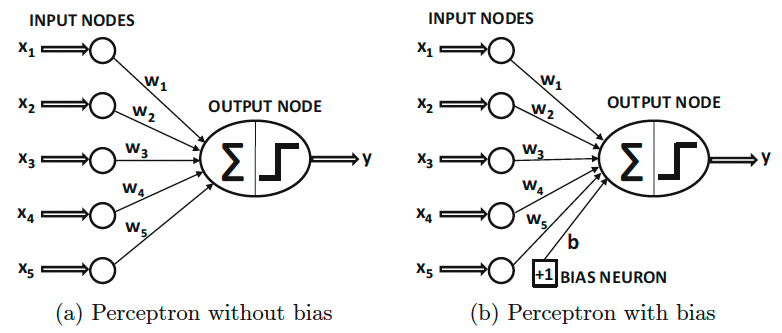
\includegraphics[width=0.85\textwidth]{./images/perceptron/basic_architecture.png}\\
        {\scriptsize \color{col:attribution} 
        Basic architecture of the perceptron. 
        Image reproduced from p.5 of \cite{Aggarwal:2018SpringerDL}}\\
    \end{center}

    It is a 
    \index{binary classification}{\bf binary classification} algorithm for 
    \index{supervised learning}{\bf supervised learning}.

\end{frame}

%
%
%

\begin{frame}[t]{What problem does the perceptron tries to solve?}

    Consider the following problem. You have:
    \begin{itemize}
        \item a {\bf vector of $d$ feature variables}, $\vect{x}$ = $(x_1, x_2, ..., x_d)^T$, and
        \item a {\bf single binary variable} $y$ ($\in$ \{-1, +1\}).   
    \end{itemize}
    The binary variable $y$ \underline{depends on} the feature variables $\vect{x}$.\\
    \vspace{0.2cm}

    \begin{blockexample}{}
        \small
        For example:
        \begin{itemize}
            \small
            \item 
                $\vect{x}$: properties of a tumor imaged using computed tomography\\ 
                $y$: is the tumor is benign or malignant?
            \item 
                $\vect{x}$: features of an event observed in a particle physics detector\\ 
                $y$: is the event a new physics candidate 
                  or Standard Model background?
            \item 
                $\vect{x}$: details about a credit card transaction, such
                   as time, amount, location, and frequency of past transactions\\
                $y$: is the transaction fraudulent?
        \end{itemize}
    \end{blockexample}

\end{frame}

%
%
%

\begin{frame}[t]{What problem does the perceptron tries to solve?}

    Consider the following problem. You have:
    \begin{itemize}
        \item a {\bf vector of $d$ feature variables}, $\vect{x}$ = $(x_1, x_2, ..., x_d)^T$, and
        \item a {\bf single binary variable} $y$ ($\in$ \{-1, +1\}).   
    \end{itemize}
    The binary variable $y$ \underline{depends on} the feature variables $\vect{x}$.\\
    \vspace{0.4cm}
    We may have a \index{training set}{\bf training set} $\mathbb{D}$ that 
    consists of several ($\vect{x}$,$y$) examples.\\
    \begin{blockexample}{}
        \small
        For instance, we may have accumulated ($\vect{x}$,$y$) examples:
        \begin{itemize}
            \small
            \item from historical observations, or
            \item from simulations
        \end{itemize}
    \end{blockexample}  
    \vspace{0.2cm}
    Can we use the training set to {\bf learn the mapping} from $\vect{x}$ to $y$?\\
    \vspace{0.2cm}
    If we knew that mapping, we could apply it to new instances of $\vect{x}$
    for which $y$ is not known and needs to be predicted.
\end{frame}

%
%
%

\begin{frame}[t]{What function does the perceptron compute?}

    Let $\hat{y}$ be our prediction of $y$ for a given feature vector $\vect{x}$.
    The \index{perceptron}\gls{perceptron} computes the prediction as follows:
    \begin{equation}
        \hat{y} = sign\Big\{ \vect{w}^T \cdot \vect{x} \Big\} = sign\Big\{ \sum_{i=1}^{d} w_i x_i \Big\}
        \label{eq:perceptron_prediction_wo_bias}
    \end{equation}        

    \vspace{-1.0cm}

    \begin{columns}
        \begin{column}{0.50\textwidth}
         \begin{center}
          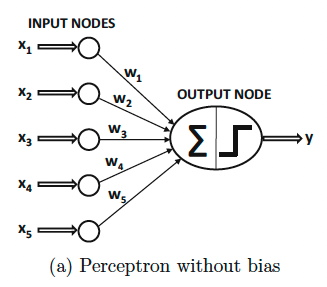
\includegraphics[width=0.95\textwidth]{./images/perceptron/perceptron_without_bias.png}\\
          {\scriptsize \color{col:attribution} 
          Image reproduced from p.5 of \cite{Aggarwal:2018SpringerDL}}\\
         \end{center}
        \end{column}
        \begin{column}{0.50\textwidth}
            \begin{itemize}
                \small
                \item Computes a linear function 
                ($\vect{w}^T \cdot \vect{x}$) in the output node.
                \item The sign function plays the role of
                an \index{activation function}\gls{activation function}.
                \item It maps a real value to either +1 or -1.
            \end{itemize}        
        \end{column}
    \end{columns}
      
\end{frame}

%
%
%

\begin{frame}[t]{What function does the perceptron compute?}

    We may need to add a \index{bias}{\bf bias} variable $b$, 
    to capture an invariant part of the prediction. 
    In this case, the \index{perceptron}\gls{perceptron} prediction is computed as follows:
    \begin{equation}
        \hat{y} = 
            sign\Big\{ \vect{w}^T \cdot \vect{x} + b \Big\} = 
            sign\Big\{ \sum_{i=1}^{d} w_i x_i + b \Big\}
            \label{eq:perceptron_prediction_w_bias}    
    \end{equation}

    \vspace{-1.0cm}

    \begin{columns}
        \begin{column}{0.50\textwidth}
         \begin{center}
            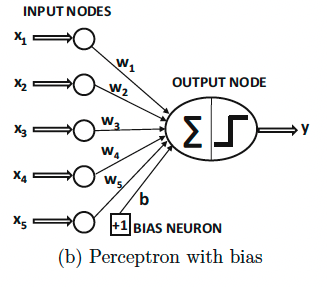
\includegraphics[width=0.95\textwidth]{./images/perceptron/perceptron_with_bias.png}\\
            {\scriptsize \color{col:attribution} 
            Image reproduced from p.5 of \cite{Aggarwal:2018SpringerDL}}\\
         \end{center}
        \end{column}
        \begin{column}{0.50\textwidth}
            \begin{itemize}
                \small
                \item Another approach to incorporate the bias, 
                is by \index{feature engineering}\gls{feature engineering}.
                \item Bias is the weight applied to an additional ($d$+1) 
                feature variable that always takes the value of 1.
                \item With that additional feature variable, 
                Eq. \ref{eq:perceptron_prediction_w_bias}
                can be reduced to Eq. \ref{eq:perceptron_prediction_wo_bias}.
                Therefore, for simplicity, will not show the bias explicitly.
            \end{itemize}        
        \end{column}
      \end{columns}

\end{frame}

%
%
%

\begin{frame}[t]{The Mark 1 perceptron}

    The \index{perceptron}perceptron was invented in 1943 
    by W.\index{McCulloch}McCulloch and W.\index{Pitts}Pitts \cite{McCulloch:1943p}.
    \begin{itemize}
      \item It is sometimes called the \index{McCulloch-Pitts neuron}\gls{McCulloch-Pitts neuron}.
    \end{itemize}

    It was first implemented \underline{in hardware} in 1958, 
    by \index{Rosenblatt}\gls{Rosenblatt} \cite{Rosenblatt:1958p}.
    \begin{itemize}
        \item It is known as the \index{Mark 1 perceptron}\gls{Mark 1 perceptron}.
      \end{itemize}
  
    \begin{columns}[t]
        \begin{column}{0.25\textwidth}
         \begin{center}
            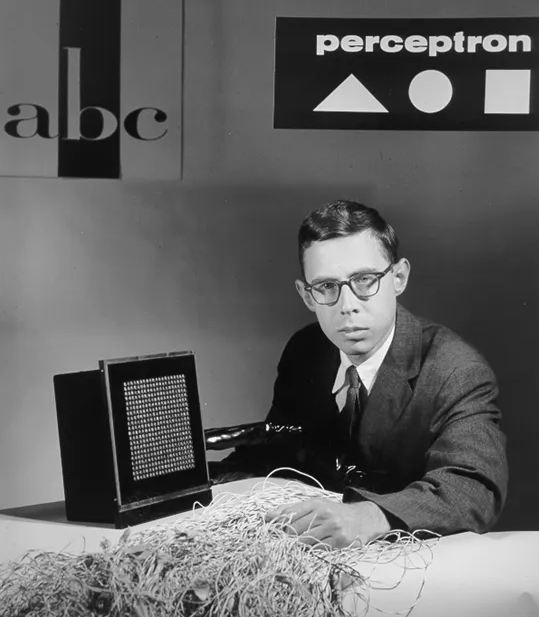
\includegraphics[width=0.95\textwidth]{./images/people/rosenblat_1.png}\\
            {\tiny 
            Rosenblatt and a part of his perceptron.\\
            \color{col:attribution} 
            Image reproduced from \cite{AIPlainEng:RiseAndFallOfPerceptron}\\}
         \end{center}
        \end{column}
        \begin{column}{0.50\textwidth}
            \begin{center}
                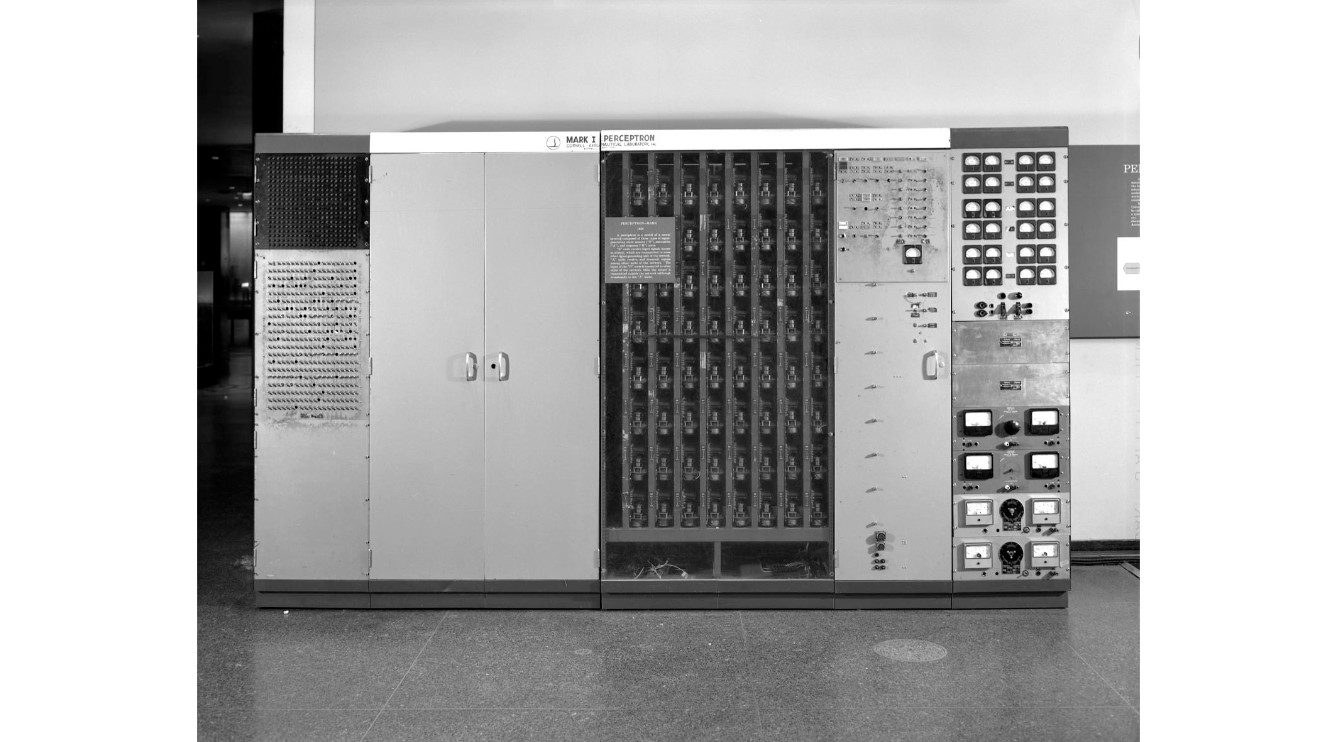
\includegraphics[width=0.98\textwidth]{./images/perceptron/mark1.png}\\
                {\tiny 
                The Mark 1 perceptron.\\
                \color{col:attribution} 
                Courtesy of The Smithsonian Institute\\ (Source: National Museum of American History)\\}
             \end{center}
        \end{column}
        \begin{column}{0.20\textwidth}
        \end{column}
      \end{columns}

\end{frame}

%
%
%

\begin{frame}[t]{The perceptron as a computational unit}

    The function computed by the \index{perceptron}\gls{perceptron},
    as well as the learning process, is similar to that of several
    other types of \index{linear model}\glspl{linear model} in \gls{ml}.
    
    The \gls{perceptron} can be seen as a {\bf computational unit}.
    
    We can combine multiple units and create more powerful models.
    
    \begin{center}
        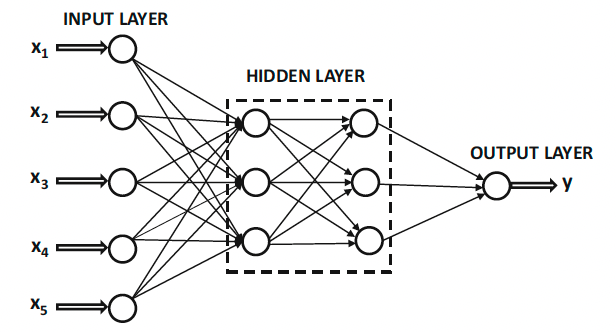
\includegraphics[width=0.70\textwidth]{./images/perceptron/combining_units.png}\\
        {\scriptsize \color{col:attribution} 
        Image reproduced from p.18 of \cite{Aggarwal:2018SpringerDL}}\\
     \end{center}
    
    
    \end{frame}

%
%
%

\begin{frame}[t]{How does the perceptron learn?}

    Our goal is to {\bf reduce the number of misclassifications}.\\
    \vspace{0.3cm}

    The error of the prediction is:
    \begin{equation}
        E(\vect{x}) = y - \hat{y}
        \label{eq:perceptron_prediction_error}
    \end{equation}        
    where $\hat{y}$ is given by Eq. \ref{eq:perceptron_prediction_wo_bias} 
    (or Eq. \ref{eq:perceptron_prediction_w_bias})\\
    \vspace{0.5cm}

    $E(\vect{x})$ takes values from the set: \{ -2, 0, +2 \}.\\
    \begin{center}
        \begin{tabular}{rrcr}
            \hline
            $y$  & $\hat{y}$ & classification & $E(\vect{x})$ \\
            \hline
            -1   & -1  &   correct &   0  \\
            -1   & +1  &   wrong   &  -2  \\
            +1   & -1  &   wrong   &  +2  \\
            +1   & +1  &   correct &   0  \\
            \hline
    \end{tabular}
    \end{center}

    If $E(\vect{x}) \ne 0$, the {\bf weights need to be updated}, but how?\\

\end{frame}

%
%
%

\begin{frame}[t]{How does the perceptron learn?}

    The learning process follows the {\em error gradient}.\\
    \vspace{0.4cm}   

    Almost all neural network learning problems are expressed in a similar way, 
    with the minimization of a suitable 
    \index{loss function}\gls{loss function} (or 
    \index{objective function}\gls{objective function}) $L$.\\
    \begin{equation}
        \vect{w} \rightarrow \vect{w^\prime} = \vect{w} - \alpha \nabla_{\vect{w}} L
        \label{eq:weight_update_grad_descent}
    \end{equation}
    where $\alpha$ regulates the learning rate.\\
    \vspace{0.4cm}

    {\color{red}grad descent}
    In the \index{perceptron}\gls{perceptron},
    as with all \index{linear model}\glspl{linear model},
    the process tries to determine the linear hyperplane: 
    \begin{equation}
        \vect{w}^T \cdot \vect{x} = 0
        \label{eq:percepton_hyperplane_1}
    \end{equation} 
    separating the training instances with $y$=+1 
    from those with $y$=-1.\\
    \vspace{0.2cm}
    \noindent\rule{4cm}{0.4pt}\\
    {\small
        Note: $\vect{w}^T \cdot \vect{x}$ 
        is the argument of the {\em sign} function computed by the 
        \index{perceptron}\gls{perceptron}.\\
    }

\end{frame}


%
%
%

\begin{frame}[t]{How does the perceptron learn?}
    
    \begin{center}
        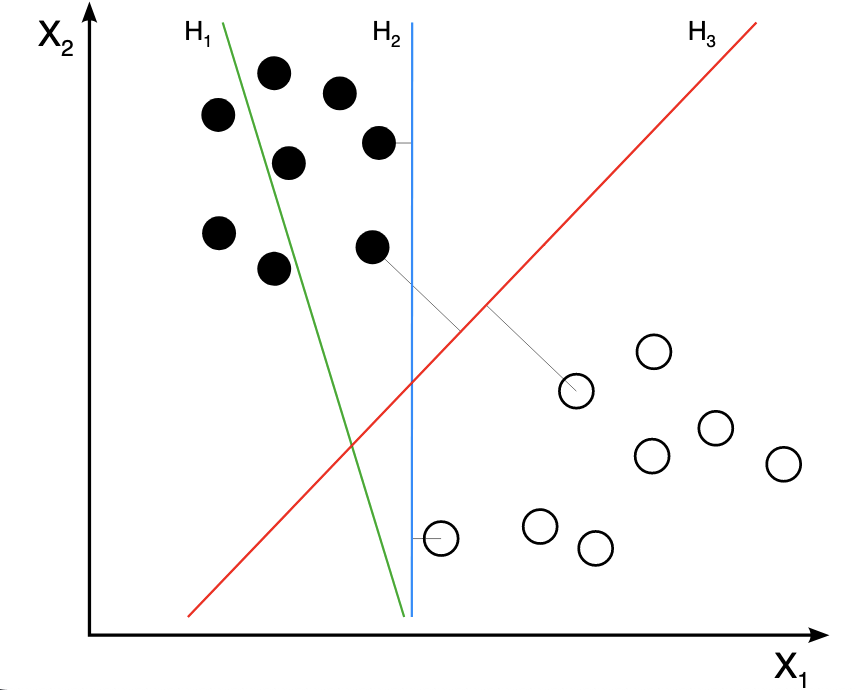
\includegraphics[width=0.55\textwidth]{./images/perceptron/data_linearly_separable.png}\\
        {\scriptsize 
        The hyperplane $H_3$ provides better separation than $H_1$ and $H_2$.
        \color{col:attribution} 
        Image reproduced from \cite{Wikipedia:LinearSeparability}}\\
    \end{center}
    \vspace{0.2cm}
    What if the data is {\bf \underline{not} linearly separable}?\\
    The \index{perceptron}\gls{perceptron} performs poorly in that case, but we will discuss this later.\\

\end{frame}



%
%
%

\begin{frame}[t]{Heuristic update process of the Mark 1 perceptron}

    As we have seen (Eq. \ref{eq:weight_update_grad_descent}), 
    the \index{perceptron}\gls{perceptron} 
    learning algorithm can be expressed as:
    \begin{equation*}
        \vect{w} \rightarrow \vect{w^\prime} = \vect{w} - \alpha \nabla_{\vect{w}} L
    \end{equation*}

    Mark 1 used a {\bf heuristic weight optimization}, performed in hardware.\\
    It was not derived from a \index{loss function}\gls{loss function} 
    using \index{gradient descent}\gls{gradient descent}.\\
    \vspace{0.2cm} 
    Updates were designed to minimize the number of misclassifications:\\
    \begin{equation}
        \vect{w} \rightarrow \vect{w^\prime} = 
        \vect{w} + \alpha \Big(y - \hat{y}\Big) \vect{x} =
        \vect{w} + \alpha E(\vect{x}) \vect{x} 
        \label{eq:percepton_weight_update_1}
    \end{equation}

    A comparison of the above equations shows that, 
    implicitly, the \index{perceptron}\gls{perceptron} 
    uses the following gradient: 
    \begin{equation}
        \nabla_{\vect{w}} L = 
          \sum_{(\vect{x},y) \in \mathbb{D}} 
          (y - \hat{y}) \vect{x}
    \label{eq:percepton_smooth_gradient_1}  
    \end{equation}


    % To better understand the \gls{perceptron}, we need to ask:\\
    % What differentiable \gls{loss function} does the 
    % \gls{perceptron} (implicitly) optimize?\\

\end{frame}



%
%
%

\begin{frame}[t,allowframebreaks]{Perceptron loss function -}

    What differentiable \gls{loss function} does the 
    \gls{perceptron} (implicitly) optimize?\\
    \vspace{0.3cm}

    A \index{gradient descent}\glshyph{gradient descent} 
    update proportional to $y-\hat{y}$, 
    is naturally caused by a squared loss function like $(y-\hat{y})^2$.\\
    \vspace{0.3cm}

    So, the \index{loss function}\gls{loss function}, $L$,
    could be expressed in a form that resembles 
    \index{least-squares}\gls{least squares} 
    \index{regression}\gls{regression}:\\
    \begin{equation}
        L(\vect{w}) = 
        \sum_{(\vect{x},y) \in \mathbb{D}} 
        \Big(y - \hat{y}(\vect{x};\vect{w})\Big)^2 =
        \sum_{(\vect{x},y) \in \mathbb{D}} 
        \Bigg(y - sign\Big\{ \vect{w}^T \cdot \vect{x} \Big\}\Bigg)^2
        \label{eq:percepton_leastsquares_loss_1}  
    \end{equation}

    Unlike in \index{least-squares}\gls{least squares} 
    \index{regression}\gls{regression},
    where the gradient of the \index{loss function}\gls{loss function} 
    is a smooth and continuous function, 
    here we have to deal with the gradient of the {\em sign} function. \\

    \framebreak

    \vspace{0.3cm}

    % Unlike in \index{least-squares}\gls{least squares} 
    % \index{regression}\gls{regression},
    % where the gradient of the \index{loss function}\gls{loss function} 
    % is a smooth and continuous function, 
    % here we have to deal with the gradient of the {\em sign} function. \\
    % \vspace{0.3cm}

    The \index{loss function}\gls{loss function} of Eq.~\ref{eq:percepton_leastsquares_loss_1}
    {\bf does not provide useful gradients}:\\ 
    \begin{itemize}
        \item It jumps between values at specific points, and
        \item it is constant over large areas of its parameter space.\\
    \end{itemize}
    \vspace{0.3cm}

    Can we replace this staircase-like function, 
    with another smooth and differentiable function 
    more suitable for \index{gradient descent}\gls{gradient descent}?\\
    \vspace{0.3cm}


\end{frame}

%
%
%

\begin{frame}[t]{Stochastic gradient descent for the perceptron}

    The basic training algorithm feeds 
    {\bf single training instances} $(\vect{x},y)$ into the network.
    For each instance, the algorithm:
    \begin{itemize}
        \item calculates the prediction $\hat{y}(\vect{x})$ 
        \item evaluates the prediction error $E(\vect{x})$ 
        from Eq.~\ref{eq:perceptron_prediction_error}
        ($E(\vect{x}) = y - \hat{y}$)
        \item updates the weights 
        using Eq.~\ref{eq:percepton_weight_update_1} 
        ($\vect{w} \rightarrow \vect{w^\prime} = \vect{w} + \alpha E(\vect{x}) \vect{x}$)
    \end{itemize}

    Non-zero updates are made only if we make mistakes. ($E(\vect{x}) \ne 0$.)\\
    \vspace{0.3cm}

    The algorithm cycles through all training instances in randomised order, 
    till convergence is achieved. 
    Each cycle is called an \index{epoch}\gls{epoch}.\\
    \vspace{0.3cm}
    
    Training instances can be used several times (training lasts several epochs).\\ 
    \vspace{0.3cm}

    This basic algorithm is a 
    \index{stochastic}\gls{stochastic} 
    \index{gradient descent}\glshyph{gradient descent} method.\\

\end{frame}


%
%
%

\begin{frame}[t]{Mini-batch stochastic gradient descent}

    It is also possible to have a training algorithm that does not 
    update the weight after a single training example was fed into the network.\\

    Weight updated can happen a small batch of examples:
    \begin{equation}
        \vect{w} \rightarrow \vect{w^\prime} = 
          \vect{w} + \alpha \sum_{(\vect{x},y) \in \mathbb{S}} E(\vect{x}) \vect{x}
        \label{eq:percepton_weight_update_minibatch_1}
      \end{equation}

\end{frame}

%
%
%

\begin{frame}[t]{Perceptron}


\end{frame}

%
%
%

\begin{frame}[t]{Perceptron criterion}

    For a binary classification problem, 
    the number of classification errors can be expressed by the
    \index{0/1 loss function}\gls{0/1 loss function}.\\
    \vspace{0.3cm}
    For a specific training example $i$, 
    ($\vect{x}_i$,$y_i$), it is written as:
    \begin{equation}
        L_{i}^{(0/1)} = 
          \frac{1}{2} \Bigg( y_i - \hat{y_i} \Bigg)^2 =
          1 - y_i sign\Big\{ \vect{w}^T \cdot \vect{x} \Big\}.
        \label{eq:percepton_01_loss_1}  
    \end{equation}

    The \index{perceptron}\gls{perceptron} updates, 
    implicitly optimize the \index{perceptron criterion}\gls{perceptron criterion}:
    \begin{equation}
        L_{i} = 
          max\Big\{0, - y_i(\vect{w}^T \cdot \vect{x}) \Big\}.
        \label{eq:percepton_criterion_1}  
    \end{equation}

    It is obtained from the \gls{0/1 loss function}, 
    by dropping the {\em sign} function and setting all negative values to 0
    (treating all correct predictions in a uniform way).

    \noindent\rule{4cm}{0.4pt}
    {\scriptsize
        \begin{equation*}
            L_{i}^{(0/1)} = 
            \frac{1}{2} \Big( y_i - \hat{y_i} \Big)^2 =
            \frac{1}{2} \Big( \cancelto{1}{y_i^2} + \cancelto{1}{\hat{y_i}^2} - 2 y_i \hat{y_i} \Big) =          
            \frac{1}{2} \Big( 2 - 2 y_i \hat{y_i} \Big) = 
            1 - y_i sign\Big\{ \vect{w}^T \cdot \vect{x} \Big\}
        \end{equation*}     
    }
    
\end{frame}

%
%
%

\begin{frame}[t]{Perceptron}


\end{frame}




%
%
%

\begin{frame}[t]{Choice of activation function}

    In the function computed by the \index{perceptron}\gls{perceptron}: 
    \begin{equation}
        \hat{y} = sign\Big\{ \vect{w}^T \cdot \vect{x} \Big\} = sign\Big\{ \sum_{i=1}^{d} w_i x_i \Big\}
    \end{equation}        
    the {\em sign} plays the role of the \index{activation function}\gls{activation function}.\\
    \vspace{0.2cm}

    Different choices can be made, 
    simulating other \index{linear model}\glspl{linear model} in \gls{ml}.
    \begin{itemize}
        \item least-squares regression
        \item support vector machine
        \item logistic regression
    \end{itemize}
    and others.

    Simple variation to the \gls{perceptron}, can capture a wide variety of optimization methods.
    We will return to this point later in the lecture.\\

\end{frame}


%
%
%

\begin{frame}[t]{Relationship with Support Vector Machines}

    A \gls{svm} is a \gls{ml} algorithm for \index{supervised learning} 
    developed by Vladimir Vapnik and colleagues at AT\&T Bell Labs 
    \cite{Vapnik:1995svm}\cite{Wikipedia:SVM}.\\

    Like the \index{perceptron}\gls{perceptron}, \gls{svm}
    is a \index{supervised learning}\gls{supervised learning} model 
    used for \index{classification}\gls{classification} 
    and \index{regression}\gls{regression} tasks.\\

    The \index{hinge loss}\gls{hinge loss} is 
    the \index{loss function}\gls{loss function}
    used by \glspl{svm}. 
    \begin{equation}
        L_{i}^{SVM} = 
          max\Big\{0, 1 - y_i(\vect{w}^T \cdot \vect{x}) \Big\}.
        \label{eq:hinge_loss_1}  
    \end{equation}

    The \index{perceptron criterion}\gls{perceptron criterion} 
    of Eq.~\ref{eq:percepton_criterion_1}, is a \underline{shifted} \gls{hinge loss}.

    The shift {\bf does not alter the gradient}, 
    but {\bf affects which points are lossless} and do not cause an update of weights.

\end{frame}

%
%
%

\begin{frame}[t]{Relationship with Support Vector Machines}

\end{frame}
